\section{Design of EvalTriage}
\label{sec:approach}

Figure~\ref{fig:approach-overview} shows the \sys workflow from run artifacts to evidence extraction, candidate factors, controlled replay, and diagnosis output.

\begin{figure*}[!t]
  \centering
  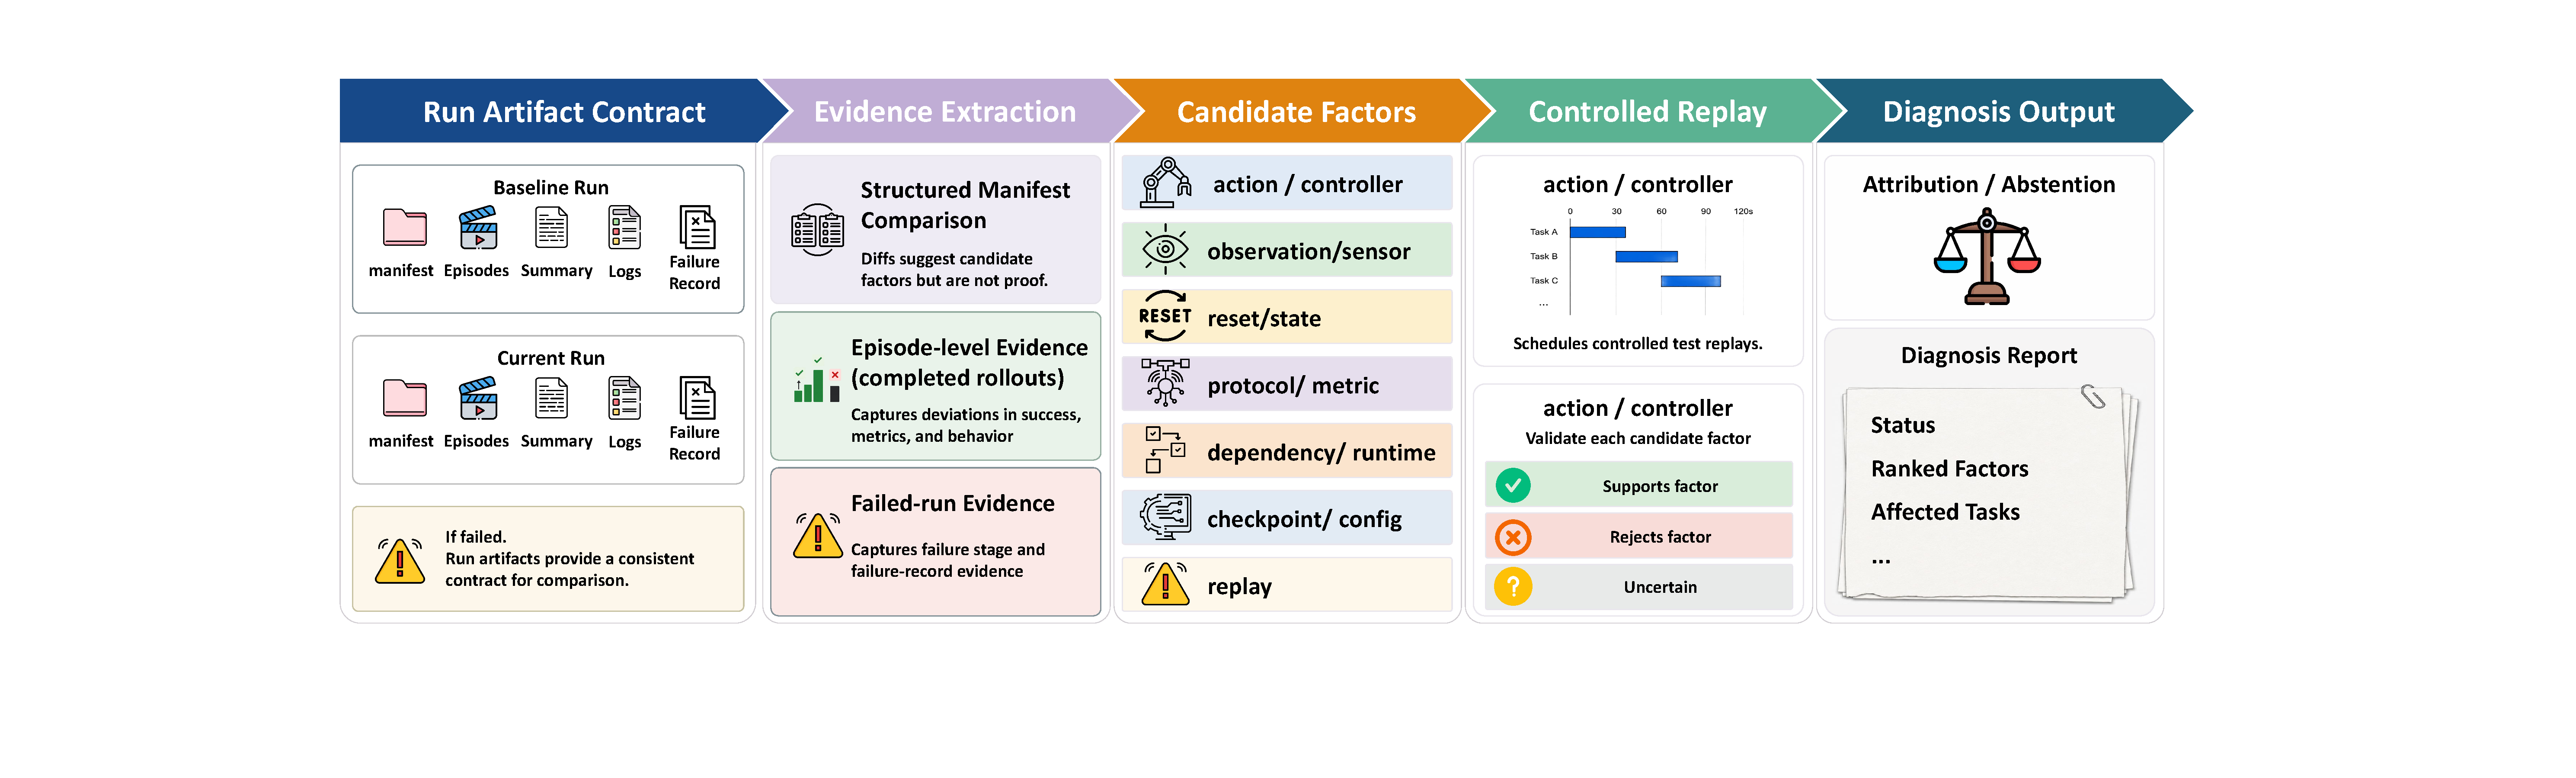
\includegraphics[width=\textwidth]{figures/fig4.pdf}
  \caption{\sys architecture: the workflow records baseline/current artifacts, extracts manifest, episode-level, and failed-run evidence, proposes candidate factors, validates them with controlled replay, and returns attribution or abstention.}
  \label{fig:approach-overview}
\end{figure*}

\subsection{Evaluation Manifest}

Each run produces a manifest that records the policy checkpoint, code version, runtime environment, task suite, seeds, evaluation protocol, observation preprocessing, action interface, reset configuration, metrics, and cost. Its fields define the candidate explanations that \sys can test. In controlled experiments, expected-factor labels and operator names are evaluation metadata, not diagnosis inputs: \sys consumes only run artifacts, manifest differences, failure records, episode outcomes, and replay outcomes, and labels are consulted only after a diagnosis is produced.

Table~\ref{tab:manifest-factors} shows how manifest fields map to factor families. The mapping is deliberately coarse enough to remain stable across projects, but concrete enough to guide replay. For example, a change in \mbox{\emph{action.control\_mode}} maps to the action/controller interface factor and can be tested by replaying with the baseline control mode. A change in task list, episode horizon, or success threshold maps to evaluation protocol/metric and can be tested by replaying the current policy under the baseline protocol. A missing processor statistic maps to checkpoint/config compatibility or observation preprocessing, depending on where the failure is observed.

\begin{table}[!t]
  \caption{Manifest Fields and Candidate Factors}
  \label{tab:manifest-factors}
  \centering
  \footnotesize
  \renewcommand{\arraystretch}{1.08}
  \begin{tabular}{@{}lp{0.56\columnwidth}@{}}
    \toprule
    Factor family & Representative manifest evidence \\
    \midrule
    Action/controller & Control mode, action scaling, postprocessing \\
    Observation/sensor & State keys, image transforms, processor stats \\
    Reset/state & Seeds, initial states, scene/task initialization \\
    Protocol/metric & Task list, episode length, success definition \\
    Dependency/runtime & Package versions, simulator backend, device \\
    Checkpoint/config & Policy checkpoint, processor, model config \\
    \bottomrule
  \end{tabular}
\end{table}

\subsection{Deviation Detection}

\sys detects deviations using aggregate metrics, failed-run status, and paired episode outcome shifts. Aggregate checks capture success-rate or reward changes. Failed-run checks capture crashes and preflight failures. Paired episode checks compare task/seed outcomes, which is important when the aggregate success rate is unchanged but the current run succeeds and fails on different episodes than the baseline.

The detector produces an evidence record rather than a binary pass/fail decision. For completed rollouts, the record includes baseline and current success rates, affected tasks, and paired episode changes. For failed runs, it includes the failing stage and the structured failure type. This record becomes the guard for attribution: if the detector does not find a thresholded deviation, \sys may still report manifest differences, but it cannot promote them to causal factors.

\subsection{Factor-Directed Replay}

Instead of blindly rerunning the benchmark, \sys plans replays that restore or control suspected factors. A replay may restore the action interface, observation pipeline, checkpoint configuration, evaluation protocol, runtime environment, dataset format, or reset behavior. The replay budget is intentionally small and targeted: it should test the most plausible factor explanation before developers repeat the benchmark.

Replay planning follows two principles. First, it preserves the comparison as much as possible: the policy, task suite, and seed remain fixed unless the suspected factor itself is one of those fields. Second, it changes only the factor being tested. This makes replay evidence interpretable. If a replay restores baseline behavior after restoring a controller interface, the controller interface becomes a supported explanation. If the replay does not recover, \sys should either try another supported factor or abstain rather than blame the most visible manifest diff without sufficient behavioral evidence.

The same idea applies to failed-run cases. A failed run may not have a success-rate drop because it does not finish. In that setting, a replay is successful when the run progresses past the failure and produces comparable artifacts. The diagnosis is therefore supported by failure recovery rather than metric recovery. This distinction is why failed-run cases are reported separately in the evaluation.

Operationally, \sys first identifies a completed-rollout or failed-run deviation, maps manifest or failure-record differences to candidate factors, and schedules a replay that tests the most plausible explanation.

\subsection{Diagnosis Rules}

\sys treats manifest and failure-record differences as hypotheses, not conclusions. A setup-sensitive attribution requires three pieces of evidence: a detected deviation, a candidate factor supported by manifest or failure evidence, and replay behavior that recovers baseline behavior or controls the failure. A factor with manifest evidence but no detected deviation is not eligible for attribution. A factor with deviation and manifest evidence but no replay support can appear as a candidate, but the diagnosis status remains unknown unless the artifact explicitly records the missing-evidence condition.

The same rules define abstention. If replay outcomes conflict, affected tasks are unstable across comparable runs, or critical artifacts are missing, \sys returns unknown rather than promoting the most visible manifest difference. This conservative rule is central to negative calibration and separates \sys from manifest-diff heuristics. Table~\ref{tab:diagnosis-statuses} lists the status vocabulary.

\begin{table}[!t]
  \caption{Diagnosis Statuses}
  \label{tab:diagnosis-statuses}
  \centering
  \renewcommand{\arraystretch}{1.08}
  \begin{tabular}{@{}p{0.30\columnwidth}p{0.64\columnwidth}@{}}
    \toprule
    Status & Meaning \\
    \midrule
    Setup-sensitive & A factor change explains the deviation through replay evidence. \\
    Flaky & Repeated comparable runs vary without a supported factor attribution. \\
    Likely true regression & Semantic code evidence remains after external-factor replays fail to explain the deviation. \\
    Unknown & Evidence is missing, weak, conflicting, or no thresholded deviation is detected. \\
    \bottomrule
  \end{tabular}
\end{table}

\subsection{Report and Artifact Contract}

The final report summarizes the affected task set, baseline/current/replay metrics, suspected factor ranking, supporting evidence, missing information, and recommended developer actions. It is meant to be inspected by developers, not only consumed as an aggregate score: a setup-sensitive report points to the recovered replay and the controlled manifest field, while an unknown report explains whether uncertainty comes from no detected deviation, missing replay, conflicting replay, or insufficient failure evidence.

\sys relies on a small file-based artifact contract between the evaluation harness and the diagnosis layer. A completed run provides a manifest, episode records, a summary file, and logs. A failed run additionally provides a failure record that states the failing stage and the exception or preflight condition. Replay runs use the same contract, which keeps baseline, current, and replay artifacts comparable and prevents diagnosis from depending on hidden process state. Table~\ref{tab:report-fields} shows the artifact fields that make the report auditable rather than purely textual.

\begin{table}[!t]
  \caption{Diagnosis Report Fields}
  \label{tab:report-fields}
  \centering
  \footnotesize
  \renewcommand{\arraystretch}{1.08}
  \begin{tabular}{@{}lp{0.60\columnwidth}@{}}
    \toprule
    Field & Purpose \\
    \midrule
    Status & Setup-sensitive, likely true regression, unknown; flaky only with repeat evidence \\
    Factor ranking & Top candidate factors and supporting evidence \\
    Affected tasks & Tasks or episodes whose outcomes changed \\
    Replay evidence & Recovery, non-recovery, or missing replay state \\
    Missing evidence & Reason for abstention or reduced confidence \\
    Cost & Episodes, reruns, graphics processing unit (GPU) minutes, and wall-clock minutes \\
    \bottomrule
  \end{tabular}
\end{table}
